\chapter{Introduction}
\label{chp:intro}
\pagenumbering{arabic}


\section{What is \GrG?}

{\scshape GrGen} (\textsc{G}raph \textsc{R}ewrite \textsc{Gen}erator) is a generative programming system for graph rewriting,
which considerably eases the transformation of complex graph structured data,
comparable to other programming tools like parser generators which ease the task of formal language recognition,
or databases which ease the task of persistent data storage and querying. 

It is combined from two groups of components:
The first consists of the compiler \texttt{grgen} -- transforming declarative graph rewrite rule specifications into highly efficient .NET-assemblies --
and the execution environment \texttt{libGr}, which offer the basic functionality of the system. 
The second consists of the interactive command line \texttt{GrShell} and the graph viewer \texttt{yComp},
which offer a rapid prototyping environment supporting graphical and stepwise debugging of programmed rule applications.

\GrG~is the successor of the \textsc{GrGen} tool presented at ICGT 2006~\cite{GBGHS:06}. 
The ``.NET'' postfix of the new name indicates that \textsc{GrGen} has been reimplemented in C\# for the Microsoft .NET or Mono environment~\cite{NET,MONO};
it is open source licensed under LGPL3 and available for download at \url{www.grgen.net}.
Starting as a compiler construction helper tool it has grown into a software development tool for general purpose graph transformation,
which offers the highest combined speed of development and execution for graph based algorithms through its declarative languages with automatic optimization.


\section{When to use \GrG~and when not}
You may be interested in using \GrG\ if you have to tackle the task of transforming meshes of massively linked objects, i.e. graph-like data structures,
as is the case in e.g. model transformation, computer linguistics, or modern compiler construction 
(any time there is more than one relation of interest in between the data entities your algorithm operates upon).
These tasks are traditionally handled by pointer structures and pointer structure navigation-, search-, and replacement routines written by hand
-- this low-level, pointer-fiddling code can be generated automatically for you by \GrG.
You specify your transformation task on a higher level of nodes connected by edges, and rewrite rules of patterns to be searched plus modifications to be carried out,
and then let \GrG\ generate the algorithmic core of your application.

There is nothing to gain from \GrG\ if scalars, lists and trees are sufficient to \emph{adequately} model your domain 
(which is the case for a lot of tasks in computing indeed; 
but which is not the case for others which would be better modeled with graphs, but aren't because of the cost of maintaining graph structures by hand).
The graph rewrite generator is not the right tool for you if you're searching for a visual environment to teach children programming -- it's a tool for software engineers.
Neither is it what you need if your graph structured data is to be interactively edited by an end user instead of being automatically transformed by rules (the editor generator DiaGen\cite{diagen} may be of interest in this case).


\section{Features of \GrG}\indexmain{features}

The process of graph rewriting can be divided into four steps:
Representing a graph according to a model (creating an instance graph), 
searching a pattern aka finding a match, 
performing changes to the matched spot in the host graph, 
and, finally, selecting which rule(s) to apply where next.
We have organized the presentation of the features of the \GrG\ languages according to this breakdown of graph rewriting:

\begin{itemize}
  \item The graph model (meta-model) language supports:
  \begin{itemize}
    \item Typed nodes and edges, with multiple inheritance on types
    \item Directed multigraphs (including multiple edges of the same type)
    \item Undirected and arbitrarily directed edges
    \item Node and edge types can be equipped with typed attributes (like structs) including powerful set and map types
    \item Connection assertions to restrict the ``shape'' of graphs
    \item Turing complete language for checking complex conditions
  \end{itemize}
  
  \item The pattern language supports:
  \begin{itemize}
    \item Plain isomorphic subgraph matching (injective mapping)
    \item Homomorphic matching for a selectable set of nodes / edges, so that the matching is not injective
    \item Attribute conditions (e.g. arithmetic-,boolean-,string- or set-expressions on the attributes)
    \item Type conditions (including powerful instanceof-like type expressions)
    \item Nested patterns, specifying negative and positive application conditions as well as iterated, optional, or alternative structures
    \item Subpatterns for pattern reuse, allowing via recursion to match substructures of arbitraty depth (e.g. iterated paths) and breadth (e.g multinodes)
    \item Parameter passing to rules
  \end{itemize}
  
  \item The rewrite language supports:
  \begin{itemize}
    \item Keeping, adding and deleting graph elements according to the SPO approach
	\item Choosing out of three additional rule application semantics: DPO or exact patterns only or induced subgraphs only
    \item Attribute re-/calculation (assigning the result of e.g. arithmetic expressions to the attributes)
    \item Retyping of nodes/edges (a more general version of casts known from common programming languages)
    \item Creation of new nodes/edges of only dynamically known types
    \item Two modes of specification: A rule can either express changes to be made to the match or replace the whole match
    \item Embedded graph rewrite sequences capable of calling other rules (with access to the nodes/edges of the rule)
    \item Emitting user-defined text to \texttt{stdout} or files during the rewrite steps
	\item A rewrite part for the nested patterns and subpatterns, so that complex structures can not only get matched, but also get rewritten
	\item Visited flags (which can be written here, in addition to reading them in the pattern language)
    \item Parameter passing out of rules
  \end{itemize}
  
  \item The rule application language (grs: graph rewrite sequences) supports:
  \begin{itemize}
    \item Composing several rules with sequential, logical, and iterative control
    \item Variables to store graph elements handed into rules and returned from rules
	\item Visited flags management
	\item Storages, i.e. sets and maps capable of storing graph elements and allowing element-wise iteration
  \end{itemize}
\end{itemize}

\noindent These were the features of the core of \GrG-System, 
the generator \texttt{grgen.exe} and its languages plus its runtime environment \texttt{libGr}.
In addition, the \GrG\ system offers a shell application, the \GrShell, 
which features commands for
\begin{table}[htbp]
    \begin{tabularx}{\linewidth}{ll}
		\hspace{12mm}-- graph management,\hspace{3cm} & -- graph validation,\\[5pt]
		\hspace{12mm}-- graph input and output, & -- graph manipulation,\\[5pt]
		\hspace{12mm}-- graph and model queries, & -- graph visualisation,\\[5pt]
		\hspace{12mm}-- action execution, & -- debugging,\\[5pt]
		\hspace{12mm}-- backend selection and usage. 
    \end{tabularx}    
%    \caption{Semantics of pattern modifiers}
    \label{tbl:overview:shellcommands}
\end{table}

The debugging and graph visualisation commands are implemented in cooperation with the graph viewer \yComp.
Alternatively to \GrShell, you can access the match and rewrite facility through \LibGr. 
This way you can build your own algorithmic rule applications in a .NET language of your choice. 


\section{System Overview}\indexmain{overview, system}

Figure~\ref{figsys} gives an overview of the \GrG\ system components. 
%Table~\ref{dirstruc} shows the \GrG\ directory structure.

\begin{figure}[htbp]
  \centering
	\scalebox{0.8}{
  \begin{tikzpicture}
      \begin{scope}[shape=rectangle,minimum size=0.75cm,text width=3cm,text centered]
          \tikzstyle{every node}=[draw]
          \node (spec1)    at (0   ,0)    {Rewrite Rules\indexmain{rewrite rule} (*\indexed{.grg})};
          \node (spec2)    at (0   ,2)    {Graph Model\indexmain{graph model} (*\indexed{.gm})};
          \node (grgen)    at (4   ,1)    {\GrG\ Generator\indexmain{generator} (Java, C\#)};
          \node (rewriter) at (10  ,0)    {Rewrite~Rules (C\#)};
          \node (types)    at (10  ,2)    {Graph~Model (C\#)};
          \node (data)     at (14  ,1)    {Graph~Management (C\#)};
          \node (libgr)    at (12  ,4)    {\LibGr\indexmain{libGr}\ (C\#)};
          \node[fill,color=gray] (app)      at (14.1  ,5.6)  {};
          \node[fill=white] (app)      at (14  ,5.5)  {Applications};
          \node (grsh)     at (10  ,5.5)  {\GrShell\indexmain{GrShell}\ (C\#)};
          \node (grs)      at (6   ,5.5)  {Graph Rewrite Script\indexmain{graph rewrite script}\indexmainsee{GrShell script}{graph rewrite script}\indexmainsee{script}{graph rewrite script} (*\indexed{.grs})};
      \end{scope}

      \node[draw, minimum width=9cm,minimum height=4cm] (engine) at (12,1) {};
      \node[draw, minimum width=9cm,minimum height=4cm,style=dotted] (ct) at (2,1) {};
      \node[anchor=north east] (engine_lab) at (engine.north east) {Backend\indexmain{backend} (Run Time)};
      \node[anchor=north east] (ct_lab) at (ct.north east) {Frontend (Compile Time)};

      \draw[->,dashed,red,>=triangle 45]     (spec1)   -> (grgen);
      \draw[->,dashed,red,>=triangle 45]     (spec2)   -> (grgen);
      \draw[->,dashed,red,>=triangle 45]     (grgen)   -> (types);
      \draw[->,line width=1pt,>=triangle 45] (grgen)   -> (engine);
      \draw[->,dashed,red,>=triangle 45]     (grgen)   -> (rewriter);
      \draw[->,line width=1pt,>=triangle 45] (app)     -> (libgr);
      \draw[->,line width=1pt,>=triangle 45] (grsh)    -> (libgr);
      \draw[->,dashed,red,>=triangle 45]     (grs)     -> (grsh);
      \draw[->,line width=1pt,>=triangle 45] (libgr)   -> (engine);

      \draw[->,line width=1pt,>=triangle 45] (-1.75,5.5) -- +(2.5,0) node[above, midway] {call};
      \draw[->,dashed,red,>=triangle 45] (-1.75,4.5)  -- +(2.5,0) node[above, midway] {read / generate};
  \end{tikzpicture}
	}
  \caption{\GrG\ system components~\cite{Kro:07}}
  \label{figsys}
\end{figure}
% DELETED, "specs" and "lib" is not applicable any more
%\begin{table}[htbp]
%  \begin{tabularx}{\linewidth}{|lX|} \hline
%  bin & Contains the .NET assemblies, in particular \indexed{GrGen.exe} (the graph rewrite system generator), \indexed{lgspBackend.dll} (a \GrG\ backend), \indexed{LibGr.dll} (the backend API), and the shell \indexed{GrShell.exe}.  \\ 
%  lib & Contains the \GrG\ generated assemblies (*.dll). \\
%  specs & Contains the graph rewrite system source documents (*.gm and *.grg). \\
%  examples & 
%  \end{tabularx}
%  \caption{\GrG\ directory structure}
%  \label{dirstruc}
%\end{table}

A graph rewrite system\footnote{In this context, system is not a CH0-like grammar rewrite system, but rather a set of interacting software components.} 
is defined by a rule set file (*.grg, which may include further rule set files) and zero or more graph model description files (*.gm). 
It is generated from these specifications by GrGen.exe and can be used by applications such as \GrShell.
Figure~\ref{process} shows the generation process.

\begin{figure}[htbp]
  \centering
	\scalebox{0.8}{
  \begin{tikzpicture}
      \begin{scope}[shape=rectangle,minimum size=0.75cm,text width=3cm,text centered]
          \tikzstyle{every node}=[draw]
          \node (gm1)      at (0   ,0)    {model1.gm};
          \node (gm2)      at (0   ,1)    {model2.gm};
          \node (gm3)      at (0   ,2)    {model3.gm};
          \node (grg)      at (4.5 ,1)    {rules1.grg};
          \node (grgen)    at (10   ,1)    {GrGen.exe};
          \node (act)      at (15.5,1) {rules1Actions.dll};
          \node (backend)  at (10   ,2)    {backend.dll};
          \node (mod)      at (15.5,2)  {rules1Model.dll};
      \end{scope}
         
			%not applicable any more
			%\draw[|-|] (-1,-1.5)   -- (5.5, -1.5)    node[below, midway] {/specs};
			%\draw[|-|] (9,-1.5)    -- (11, -1.5)     node[below, midway] {/bin};
			%\draw[|-|] (14.5,-1.5) -- (16.5, -1.5)   node[below, midway] {/lib};

      \draw[->,line width=1pt,>=triangle 45]     (grg)     -> (gm1);
      \draw[->,line width=1pt,>=triangle 45]     (grg)     -> (gm2);
      \draw[->,line width=1pt,>=triangle 45]     (grg)     -> (gm3);
      \draw[->,dashed,red,>=triangle 45]         (grg)     -> (grgen);
      \draw[->,dashed,red,>=triangle 45]         (grgen)   -> (mod);
      \draw[->,dashed,red,>=triangle 45]         (grgen)   -> (act);
      \draw[->,line width=1pt,>=triangle 45]     (mod)     -> (backend);
      \draw[->,line width=1pt,>=triangle 45]     (act)     -> (backend);


      \draw[->,line width=1pt,>=triangle 45] (-1.25,3.5) -- +(2.5,0) node[above, midway] {referencing};
      \draw[->,dashed,red,>=triangle 45]     (3.25,3.5)  -- +(2.5,0) node[above, midway] {read / generate};
  \end{tikzpicture}
	}
  \caption{Generating a graph rewrite system}
  \label{process}
\end{figure}

In general you have to distinguish carefully between a graph model (meta level), a host graph, a pattern graph and a rewrite rule.
In \GrG\ pattern graphs are implicitly defined by rules, i.e.\ each rule defines its pattern.
On the technical side, specification documents for a graph rewrite system can be available as source documents for graph models and rule sets (plain text *.gm and *.grg files) or as their translated .NET modules, either C\# source files or their compiled assemblies (*.dll).

Generating a \GrG\ graph rewrite system may be considered a preliminary task.
The actual process of rewriting as well as dealing with host graphs is performed by \GrG's backend.
\GrG\ provides a backend \indexed{API} in two versions --- the named and typed entities which get generated plus the name string and object based interface offered by the .NET library \LibGr.
For most issues---in particular for experimental purposes---you might rather want to work with the \GrShell\ because of its rapid prototyping support.
However, \GrShell\ does not provide the full power of the \LibGr; see also note~\ref{note:indeterminism} on page~\pageref{note:indeterminism}.


\section{What is Graph Rewriting?}\indexmain{graph rewriting}
\label{ov:whatsallabout}

The notion of graph rewriting as understood by \GrG\ is a method for declaratively specifying ``changes'' to a graph.
This is comparable to the well-known term rewriting. 
Normally you use one or more \newterm{graph rewrite rules} to accomplish a certain task.
\GrG\ implements an SPO-based approach (as default).
In the simplest case such a graph rewrite rule consists of a tuple $L \rightarrow R$, whereas $L$---the \newterm{left hand side}\indexmainsee{LHS}{left hand side} of the rule---is called \newterm{pattern graph} and $R$---the \newterm{right hand side}\indexmainsee{RHS}{right hand side} of the rule---is the \newterm{replacement graph}.

\begin{figure}[htbp]
	\centering
  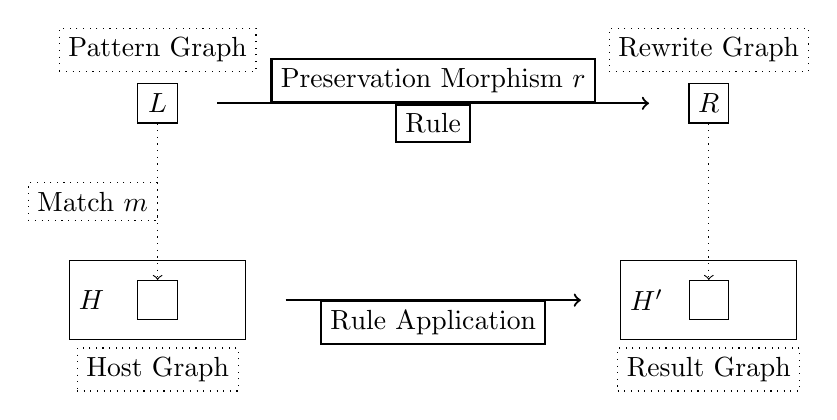
\begin{tikzpicture}
    \begin{scope}[minimum size=0.5cm]
      \tikzstyle{every node}=[draw]
      \node (L)     at (0   ,2.5) {$L$};
      \node (R)     at (7   ,2.5) {$R$};
      \node (mL)    at (0   ,0) {};
      \node (mR)    at (7   ,0) {};
      \node[text width=2cm,text badly ragged,minimum size=1cm] (H)     at (0   ,0) {$H$};
      \node[text width=2cm,text badly ragged,minimum size=1cm] (Hs)    at (7   ,0) {$H'$};
    \end{scope}

    \draw[dotted,->] (L) node[above=0.4cm] {Pattern Graph} -> (mL) node[left,midway]  {Match $m$}   node[below=0.6cm] {Host Graph};
    \draw[dotted,->] (R) node[above=0.4cm] {Rewrite Graph} -> (mR)                              node[below=0.6cm] {Result Graph};

    \pgfsetshortenstart{0.5cm}
    \pgfsetshortenend{0.5cm}
    \draw[thick,->]  (L) -> (R)  node[above,midway] {Preservation Morphism $r$} node[below,midway] {Rule};
    \draw[thick,->]  (H) -> (Hs) node[below,midway] {Rule Application};
  \end{tikzpicture}
  \caption{Basic Idea of Graph Rewriting}
  \label{figrule}
\end{figure}

Moreover we need to identify graph elements (nodes or edges) of $L$ and $R$ for preserving them during rewrite. 
This is done by a \newterm{preservation morphism} $r$ mapping elements from $L$ to $R$; the morphism $r$ is injective, but needs to be neither surjective nor total.
Together with a rule name $p$ we have $p : L \xrightarrow{r} R$.

The transformation is done by \newterm{application}\indexmainsee{rule application}{application} of a rule to a \newterm{host graph} $H$.
To do so, we have to find an occurrence of the pattern graph in the host graph. 
Mathematically speaking, such a \newterm{match} $m$ is an isomorphism from $L$ to a subgraph of $H$.
This morphism may not be unique, i.e.\ there may be several matches.
Afterwards we change the matched \indexed{spot} $m(L)$ of the host graph, such that it becomes an isomorphic subgraph of the replacement graph $R$.
Elements of $L$ not mapped by $r$ are deleted from $m(L)$ during rewrite.
Elements of $R$ not in the image of $r$ are inserted into $H$, all others (elements that are mapped by $r$) are retained.
The outcome of these steps is the resulting graph $H'$. In symbolic language: $H \xRightarrow{m, p} H'$.


\section{An Example}\indexmain{example}
\label{ov:example}

We'll have a look at a small example. 
Graph elements (nodes and edges) are labeled with and identifier.
If a type is necessary then it is stated after a colon.
We start using a special case to construct our host graph: an \indexed{empty pattern} always produces exactly one\footnote{Because of the uniqueness of the total and totally undefined morphism.} match (independent of the host graph). So we construct an apple by applying
\[
  p_0:  
  \begin{array}[c]{c} 
    \emptyset
  \end{array} 
  \begin{array}[c]{c} 
    \longrightarrow 
  \end{array} 
  \begin{array}[c]{c} 
    \begin{tikzpicture}[show background rectangle]
      \tikzstyle{every node}=[circle]
      \node[draw] (n1) at (2.5,5) {};
      \node[draw] (n2) at (2,4)   {};
      \node[draw] (n3) at (0,2)   {};
      \node[draw] (n4) at (2,0)   {};
      \node[draw] (n5) at (4,2)   {};
    	
    	\draw[-latex] (n2) --                                  (n1) node[left,midway]  {$e_1$};
    	\draw[-latex] (n2) .. controls +(-1,1) and +(0,1) ..   (n3) node[left,midway]  {$e_2$};
      \draw[-latex] (n3) .. controls +(0,-1) and +(-1,0) ..  (n4) node[left,midway]  {$e_3$};
    	\draw[-latex] (n4) .. controls +(1,0)  and +(0,-1) ..  (n5) node[right,midway] {$e_4$};
      \draw[-latex] (n5) .. controls +(0,1)  and +(1,1) ..   (n2) node[right,midway] {$e_5$};
    \end{tikzpicture}
  \end{array}
\]
to the empty host graph. 
As the result we get an apple as new host graph $H$. 
Now we want to rewrite our apple with stem to an apple with a leaflet. 
So we apply
\[
  p_1:
  \begin{array}[c]{c}
    \begin{tikzpicture}[show background rectangle]
      \tikzstyle{every node}=[circle,minimum size=0.7cm]
      \node[draw] (a) at (2,5.5)  {a};
      \node[draw] (b) at (2,4)    {b};
    	
    	\draw[-latex] (b) -- (a) node[left,midway]  {$x$};
    \end{tikzpicture}
  \end{array}
  \begin{array}[c]{c}
    \longrightarrow
  \end{array}
  \begin{array}[c]{c}
    \begin{tikzpicture}[show background rectangle]
      \tikzstyle{every node}=[circle,minimum size=0.7cm]
      \node[draw] (c) at (2,5.5)  {c};
      \node[draw] (b) at (2,4)    {b};
    	
    	\draw[-latex] (b) .. controls +(-0.7,+0.7) and +(-0.7,-0.7) .. (c) node[left,midway]   {$y$};
    	\draw[-latex] (b) .. controls +(+0.7,+0.7) and +(+0.7,-0.7) .. (c) node[right,midway]  {$z$};
    \end{tikzpicture}
  \end{array} 
\]
to $H$ and get the new host graph $H_1$, something like this:
\[
  \begin{array}[c]{c} 
    \begin{tikzpicture}[show background rectangle]
      \tikzstyle{every node}=[circle]
      \node[draw] (n1) at (2.5,5) {};
      \node[draw] (n2) at (2,4)   {};
      \node[draw] (n3) at (0,2)   {};
      \node[draw] (n4) at (2,0)   {};
      \node[draw] (n5) at (4,2)   {};
    	
    	\draw[-latex] (n2) --                                  (n1) node[left,midway]  {$e_1$};
    	\draw[-latex] (n2) .. controls +(-1,1) and +(0,1) ..   (n3) node[left,midway]  {$e_2$};
      \draw[-latex] (n3) .. controls +(0,-1) and +(-1,0) ..  (n4) node[left,midway]  {$e_3$};
    	\draw[-latex] (n4) .. controls +(1,0)  and +(0,-1) ..  (n5) node[right,midway] {$e_4$};
      \draw[-latex] (n5) .. controls +(0,1)  and +(1,1) ..   (n2) node[right,midway] {$e_5$};
    \end{tikzpicture}
  \end{array} 
  \begin{array}[c]{c} 
    \xRightarrow{\quad p_1 \quad}
  \end{array} 
  \begin{array}[c]{c} 
    \begin{tikzpicture}[show background rectangle]
      \tikzstyle{every node}=[circle]
      \node[draw] (n1) at (2.5,5) {};
      \node[draw] (n2) at (2,4)   {};
      \node[draw] (n3) at (0,2)   {};
      \node[draw] (n4) at (2,0)   {};
      \node[draw] (n5) at (4,2)   {};
      \node[draw] (n6) at (0,0.5)   {};
    	
    	\draw[-latex] (n2) --                                  (n1) node[left,midway]  {$e_1$};
    	\draw[-latex] (n2) .. controls +(-1,1) and +(0,1) ..   (n3) node[left,midway]  {$e_2$};
      \draw[-latex] (n3) .. controls +(-0.7,-0.7) and +(-0.7,+0.7) .. (n6) node[left,midway]  {$e_6$};
      \draw[-latex] (n3) .. controls +(+0.7,-0.7) and +(+0.7,+0.7) .. (n6) node[right,midway] {$e_7$};
    	\draw[-latex] (n4) .. controls +(1,0)  and +(0,-1) ..  (n5) node[right,midway] {$e_4$};
      \draw[-latex] (n5) .. controls +(0,1)  and +(1,1) ..   (n2) node[right,midway] {$e_5$};
    \end{tikzpicture}
  \end{array}
\]
What happened? 
\GrG\ has arbitrarily chosen one match out of the set of possible matches, because $x$ matches edge $e_3$ as well as $e_1$.
A correct solution could make use of edge type information. 
We have to change rule $p_0$ to generate the edge $e_1$ with a special type ``stem''.
And this time we will even keep the stem. 
So let
\[
  p_2:
  \begin{array}[c]{c}
    \begin{tikzpicture}[show background rectangle]
      \tikzstyle{every node}=[circle,minimum size=0.7cm]
      \node[draw] (a) at (2,5.5)  {a};
      \node[draw] (b) at (2,4)    {b};
    	
    	\draw[-latex] (b) -- (a) node[left,midway]  {$x:\text{stem}$};
    \end{tikzpicture}
  \end{array}
  \begin{array}[c]{c}
    \longrightarrow
  \end{array}
  \begin{array}[c]{c}
    \begin{tikzpicture}[show background rectangle]
      \tikzstyle{every node}=[circle,minimum size=0.7cm]
      \node[draw] (c) at (2,5.5)  {c};
      \node[draw] (b) at (2,4)    {b};
      \node[draw] (a) at (3.5,5.5){a};
    	
    	\draw[-latex] (b) -- (a) node[right,midway]  {$x$};
    	\draw[-latex] (b) .. controls +(-0.7,+0.7) and +(-0.7,-0.7) .. (c) node[left,midway]   {$y$};
    	\draw[-latex] (b) .. controls +(+0.7,+0.7) and +(+0.7,-0.7) .. (c) node[above,midway]  {$z$};
    \end{tikzpicture}
  \end{array}.
\]
If we apply $p_2$ to the modified $H_1$ this leads to
\[
  \begin{array}[c]{c} 
    \begin{tikzpicture}[show background rectangle]
      \tikzstyle{every node}=[circle]
      \node[draw] (n1) at (2.5,5) {};
      \node[draw] (n2) at (2,4)   {};
      \node[draw] (n3) at (0,2)   {};
      \node[draw] (n4) at (2,0)   {};
      \node[draw] (n5) at (4,2)   {};
    	
    	\draw[-latex] (n2) --                                  (n1) node[left,pos=0.8]  {$e_1:\text{stem}$};
    	\draw[-latex] (n2) .. controls +(-1,1) and +(0,1) ..   (n3) node[left,midway]  {$e_2$};
      \draw[-latex] (n3) .. controls +(0,-1) and +(-1,0) ..  (n4) node[left,midway]  {$e_3$};
    	\draw[-latex] (n4) .. controls +(1,0)  and +(0,-1) ..  (n5) node[right,midway] {$e_4$};
      \draw[-latex] (n5) .. controls +(0,1)  and +(1,1) ..   (n2) node[right,midway] {$e_5$};
    \end{tikzpicture}
  \end{array} 
  \begin{array}[c]{c} 
    \xRightarrow{\quad p_2 \quad}
  \end{array} 
  \begin{array}[c]{c} 
    \begin{tikzpicture}[show background rectangle]
      \tikzstyle{every node}=[circle]
      \node[draw] (n1) at (3,5) {};
      \node[draw] (n2) at (2,4)   {};
      \node[draw] (n3) at (0,2)   {};
      \node[draw] (n4) at (2,0)   {};
      \node[draw] (n5) at (4,2)   {};
      \node[draw] (n6) at (2,5.0)   {};
    	
    	\draw[-latex] (n2) --                                  (n1) node[right,pos=0.6] {$e_1:\text{stem}$};
    	\draw[-latex] (n2) .. controls +(-1,1) and +(0,1) ..   (n3) node[left,midway]  {$e_2$};
      \draw[-latex] (n3) .. controls +(0,-1) and +(-1,0) ..  (n4) node[left,midway]  {$e_3$};
    	\draw[-latex] (n4) .. controls +(1,0)  and +(0,-1) ..  (n5) node[right,midway] {$e_4$};
      \draw[-latex] (n5) .. controls +(0,1)  and +(1,1) ..   (n2) node[right,midway] {$e_5$};
    	\draw[-latex] (n2) .. controls +(-0.3,+0.3) and +(-0.3,-0.3) .. (n6) node[left,midway]   {};
    	\draw[-latex] (n2) .. controls +(+0.3,+0.3) and +(+0.3,-0.3) .. (n6) node[right,midway]  {};
    \end{tikzpicture}
  \end{array}.
\]


%\section{What is it good for?}
%Benefits. When to use graph rewriting. When not. TODO!


\section{The Tools}

All the programs and libraries of \GrG\ are licensed under \indexed{LGPL}. 
Notice that the \yComp\ graph viewer is not a part of \GrG ; \yComp\ ships with its own license. 
Although \yComp\ is not free software, it's free for use in academic and non-commercial areas.
You'll find the tools in the \texttt{bin} subdirectory of your \GrG\ installation.

%\pagebreak

\subsection{\texttt{\indexed{GrGen.exe}}}

\parpic[l] {

\includegraphics[width=48pt]{fig/grgen-256.png}
}
\noindent The \texttt{GrGen.exe} assembly implements the \GrG\ generator. 
The \GrG\ generator parses a rule set and its model files and compiles them into .NET assemblies.
The compiled assemblies form a specific graph rewriting system together with the \GrG\ backend.

\begin{description}
  \item[Usage] \begin{tabular*}{\linewidth}{@{}l@{}l}\texttt{[mono] GrGen.exe } & \texttt{[-keep [<dest-dir>]] [-use <existing-dir>] [-debug]}\\
        &\texttt{[-b <backend-dll>] [-o <output-dir>] <rule-set>}\end{tabular*}
    \emph{rule-set} is a file containing a rule set specification according to Chapter~\ref{chaprulelang}. Usually such a file has the suffix \texttt{\indexed{.grg}}. The suffix \texttt{.grg} may be omitted.
By default \GrG\ tries to write the compiled assemblies into the same directory as the rule set file. This can be changed by the optional parameter \emph{output-dir}.
  \item[Options] \mbox{} 
    \begin{tabularx}{\linewidth}{lX}
      \texttt{-keep} & Keep the generated C\# source files. If \emph{dest-dir} is omitted, a subdirectory \texttt{tmpgrgen$n$}\footnote{$n$ is an increasing number.} within the current directory will be created. The destination directory contains:
\begin{itemize}
  \item \texttt{printOutput.txt}---a snapshot of \texttt{stdout} during program execution.
  \item \emph{Name}\texttt{Model.cs}---the C\# source file(s) of the \emph{rule-set}\texttt{Modell.dll} assembly.
  \item \emph{Name}\texttt{Actions\_intermediate.cs}---a preliminary version of the C\# source file of the \emph{rule-set}'s actions assembly. 
	This file is for internal debug purposes only (it contains the frontend actions output).
  \item \emph{Name}\texttt{Actions.cs}---the C\# source file of the \emph{rule-set}\texttt{Actions.dll} assembly.
\end{itemize}\\
      \texttt{-use} & Don't re-generate C\# source files. Instead use the files in \emph{existing-dir} to build the assemblies.\\	
      \texttt{-debug} & Compile the assemblies with debug information.\\
      \texttt{-b} & Use the backend library \emph{backend-dll} (default is LGSPBackend).\\
      \texttt{-o} & Store generated assemblies in \emph{output-dir}.
    \end{tabularx}
  \item[Requires] .NET 2.0 (or above) or Mono 1.2.3 (or above). Java Runtime Environment 1.5 (or above).
\end{description}

\begin{note}
Regarding the column information in the error reports of the compiler please note that tabs count as one character.
\end{note}

\begin{note}\label{note:modelruledump}
The grgen compiler consists of a Java frontend used by the C\# backend \texttt{grgen.exe}.
The java frontend can be executed itself to get a visualization of the model and the rewrite rules,
in the form of a dump of the compiler IR as a .vcg file:\\
\texttt{java -jar grgen.jar -i yourfile.grg}
\end{note}


\subsection{\texttt{\indexed{GrShell.exe}}}

\parpic[l] {

\includegraphics[width=48pt]{fig/grshell-256.png}
}
\noindent The \texttt{GrShell.exe}\indexmain{GrShell} is a shell application on top of the \LibGr. 
\GrShell\ is capable of creating, manipulating, and dumping graphs as well as performing graph rewriting with graphical debug support. 
For further information about the \GrShell\ language see Chapter~\ref{chapgrshell}.

\begin{description}
  \item[Usage] \texttt{[mono] grShell.exe [-N] [-C "<commands>"] <grshell-script>*} \\
     Opens the interactive shell. The \GrShell\ will include and execute the commands in the optional list of \emph{grshell-script}s\indexmain{graph rewrite script} (usually \texttt{*\indexed{.grs}} files) in the given order.
	 The \texttt{grs} suffixes may be omitted. \GrShell\ returns 0 on successful execution, or in non-interactive mode -1 if the specified shell script could not be executed, or -2 if a \texttt{validate} with \texttt{exitonfailure} failed.
  \item[Options] \mbox{} 
    \begin{tabularx}{\linewidth}{lX}
      \texttt{-N} & Enables non-debug non-gui mode which exits on error with an error code instead of waiting for user input.\\
      \texttt{-C} & Execute the quoted \GrShell\ commands immediately (before the first script file). Instead of a line break use a double semicolon \texttt{;;} to separate commands.
    \end{tabularx}
  \item[Requires] .NET 2.0 (or above) or Mono 1.2.3 (or above).
\end{description}

\subsection{\texttt{LibGr.dll}}
\label{sct:API}
The \LibGr\indexmain{libGr} is a .NET assembly implementing \GrG's \indexed{API}.
See the extracted HTML documentation for interface descriptions at \url{http://www.grgen.net/doc/libGr/};
a short introduction is given in chaper \ref{cha:api}. 

\subsection{\texttt{yComp.jar}}
\label{tools:ycomp}
\yComp\indexmain{yComp} \cite{ycomp} is a graph visualization tool based on \yFiles\ \cite{yfiles}. 
It is well integrated and shipped with \GrG, but it's not a part of \GrG.
\yComp\ implements several graph layout algorithms and has file format support for \indexed{VCG}, GML and YGF among others. 
\begin{description}
  \item[Usage] Usually \yComp\ will be loaded by the \GrShell. You might want to open \yComp\ manually by typing\\
   \texttt{java -jar yComp.jar [<graph-file>]}\\
  Or by executing the batch file \texttt{ycomp} under Linux / \texttt{ycomp.bat} under Windows, 
  which will start \yComp\ on the given file with increased heap space. 
  The \emph{graph-file} may be any graph file in a supported format. \yComp\ will open this file on startup.
  \item[Hints] The \indexed{layout algorithm}\indexmainsee{layout}{layout algorithm} \indexedsee{compiler graph}{layout algorithm} (\yComp's default setting, a version of (\texttt{\indexedsee{hierarchic}{layout algorithm}} optimized for graph based compiler intermediate representations) may not be a good choice for your graph at hand. 
  Instead \texttt{\indexedsee{organic}{layout algorithm}} or \texttt{\indexedsee{orthogonal}{layout algorithm}} might be worth trying). 
  Use the rightmost blue play button to start the layout process. Depending on the graph size this may take a while.
\begin{center}
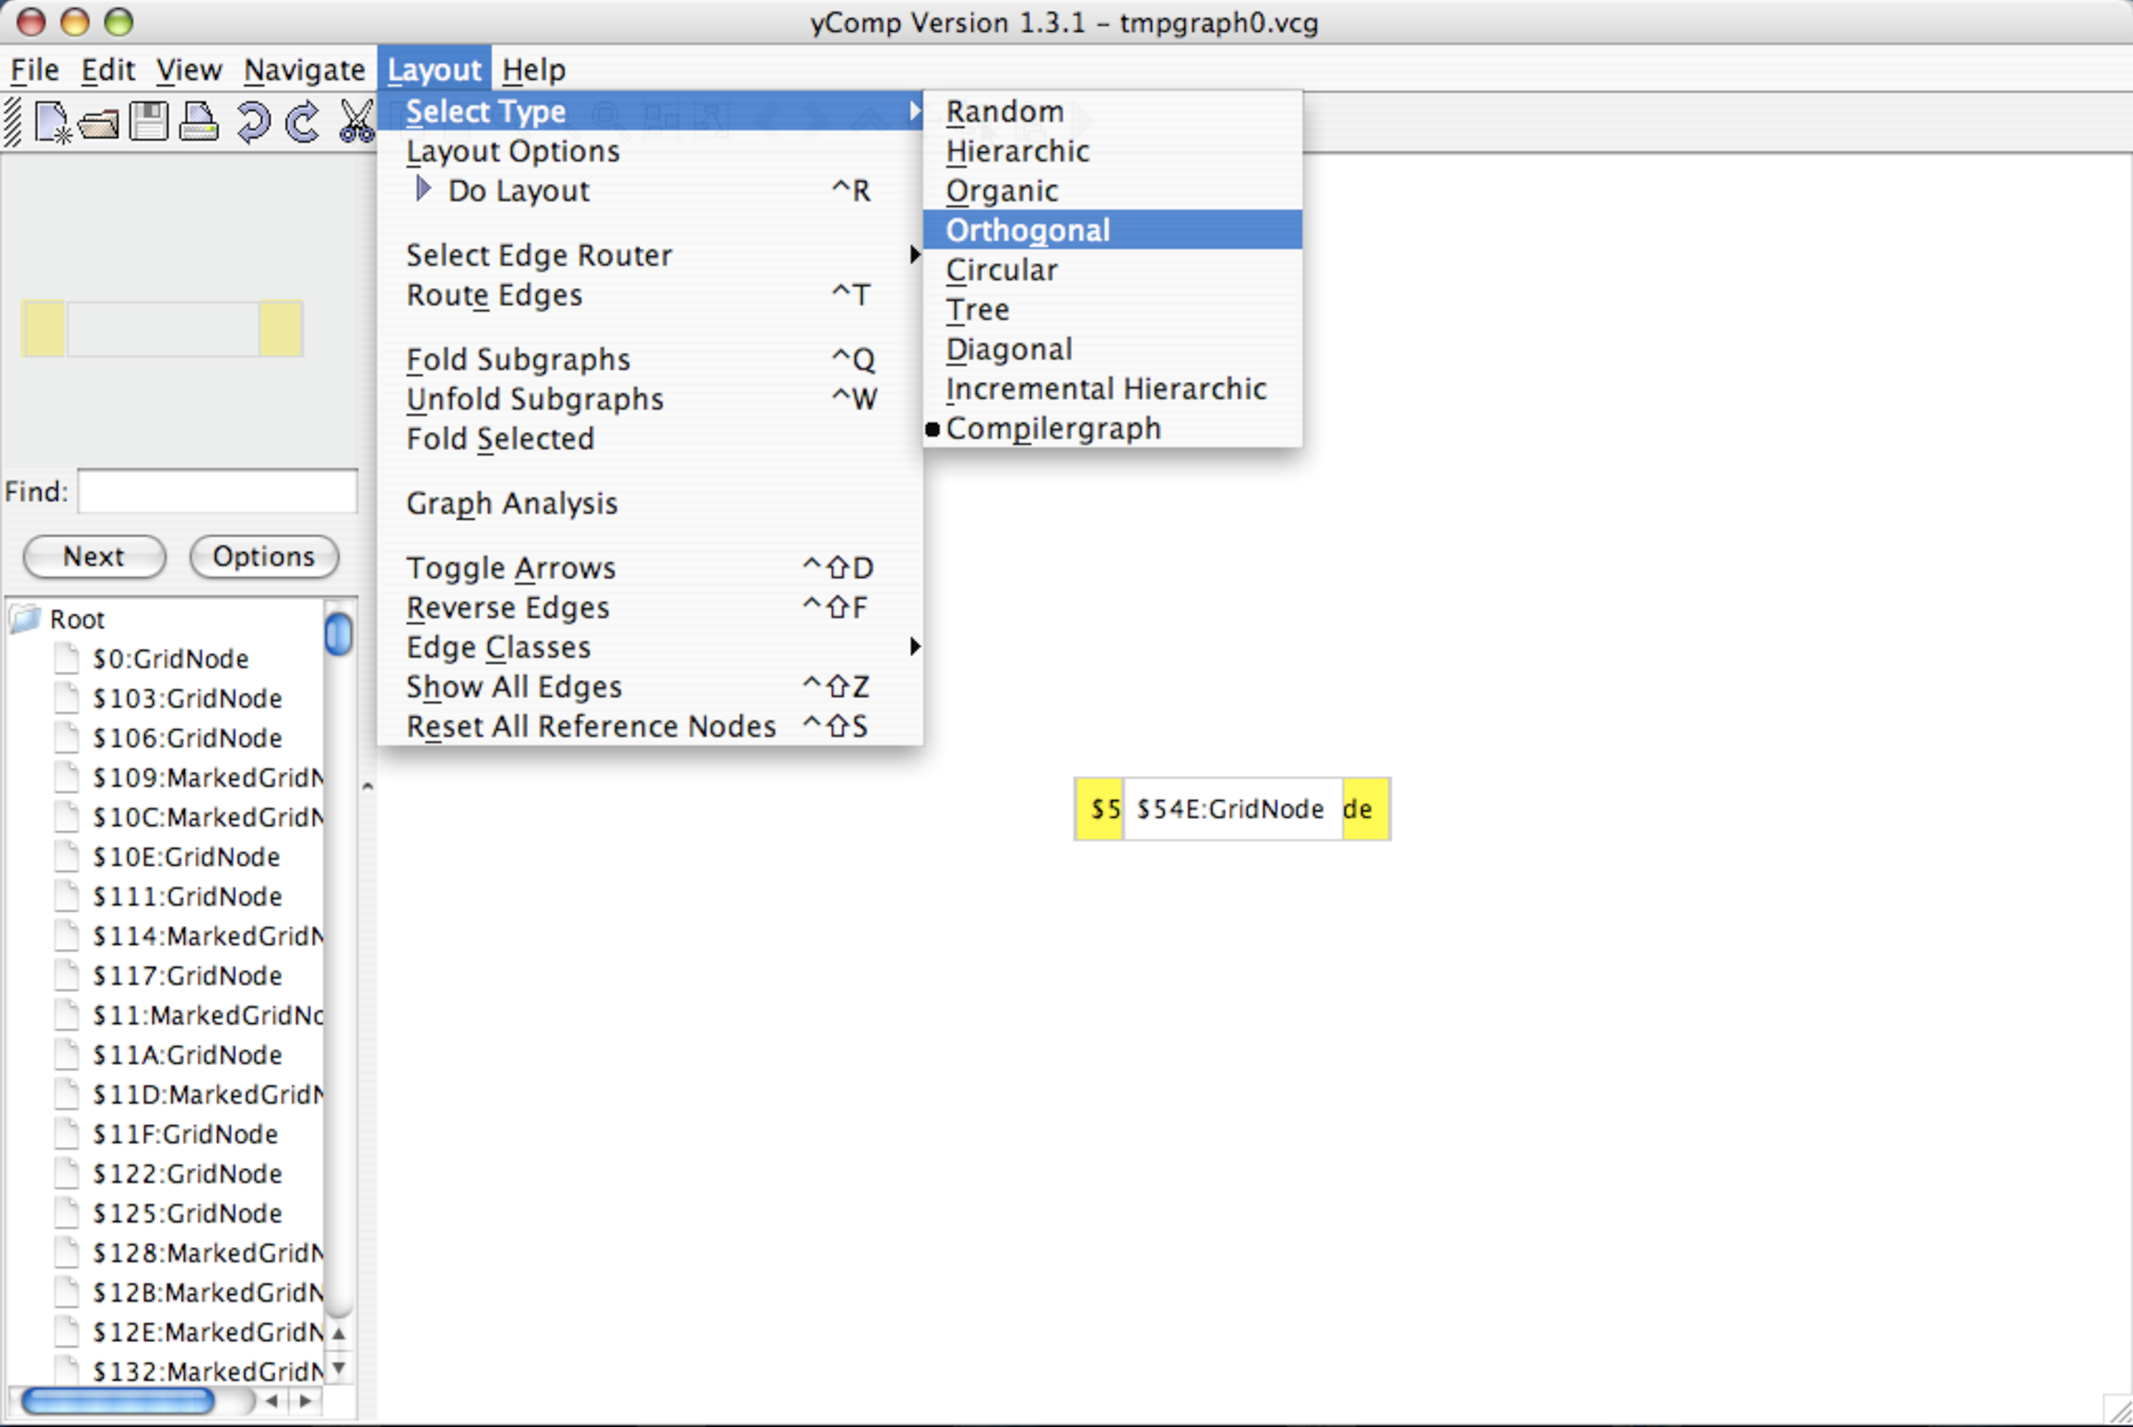
\includegraphics[width=0.45\linewidth]{fig/ycomp1.pdf} 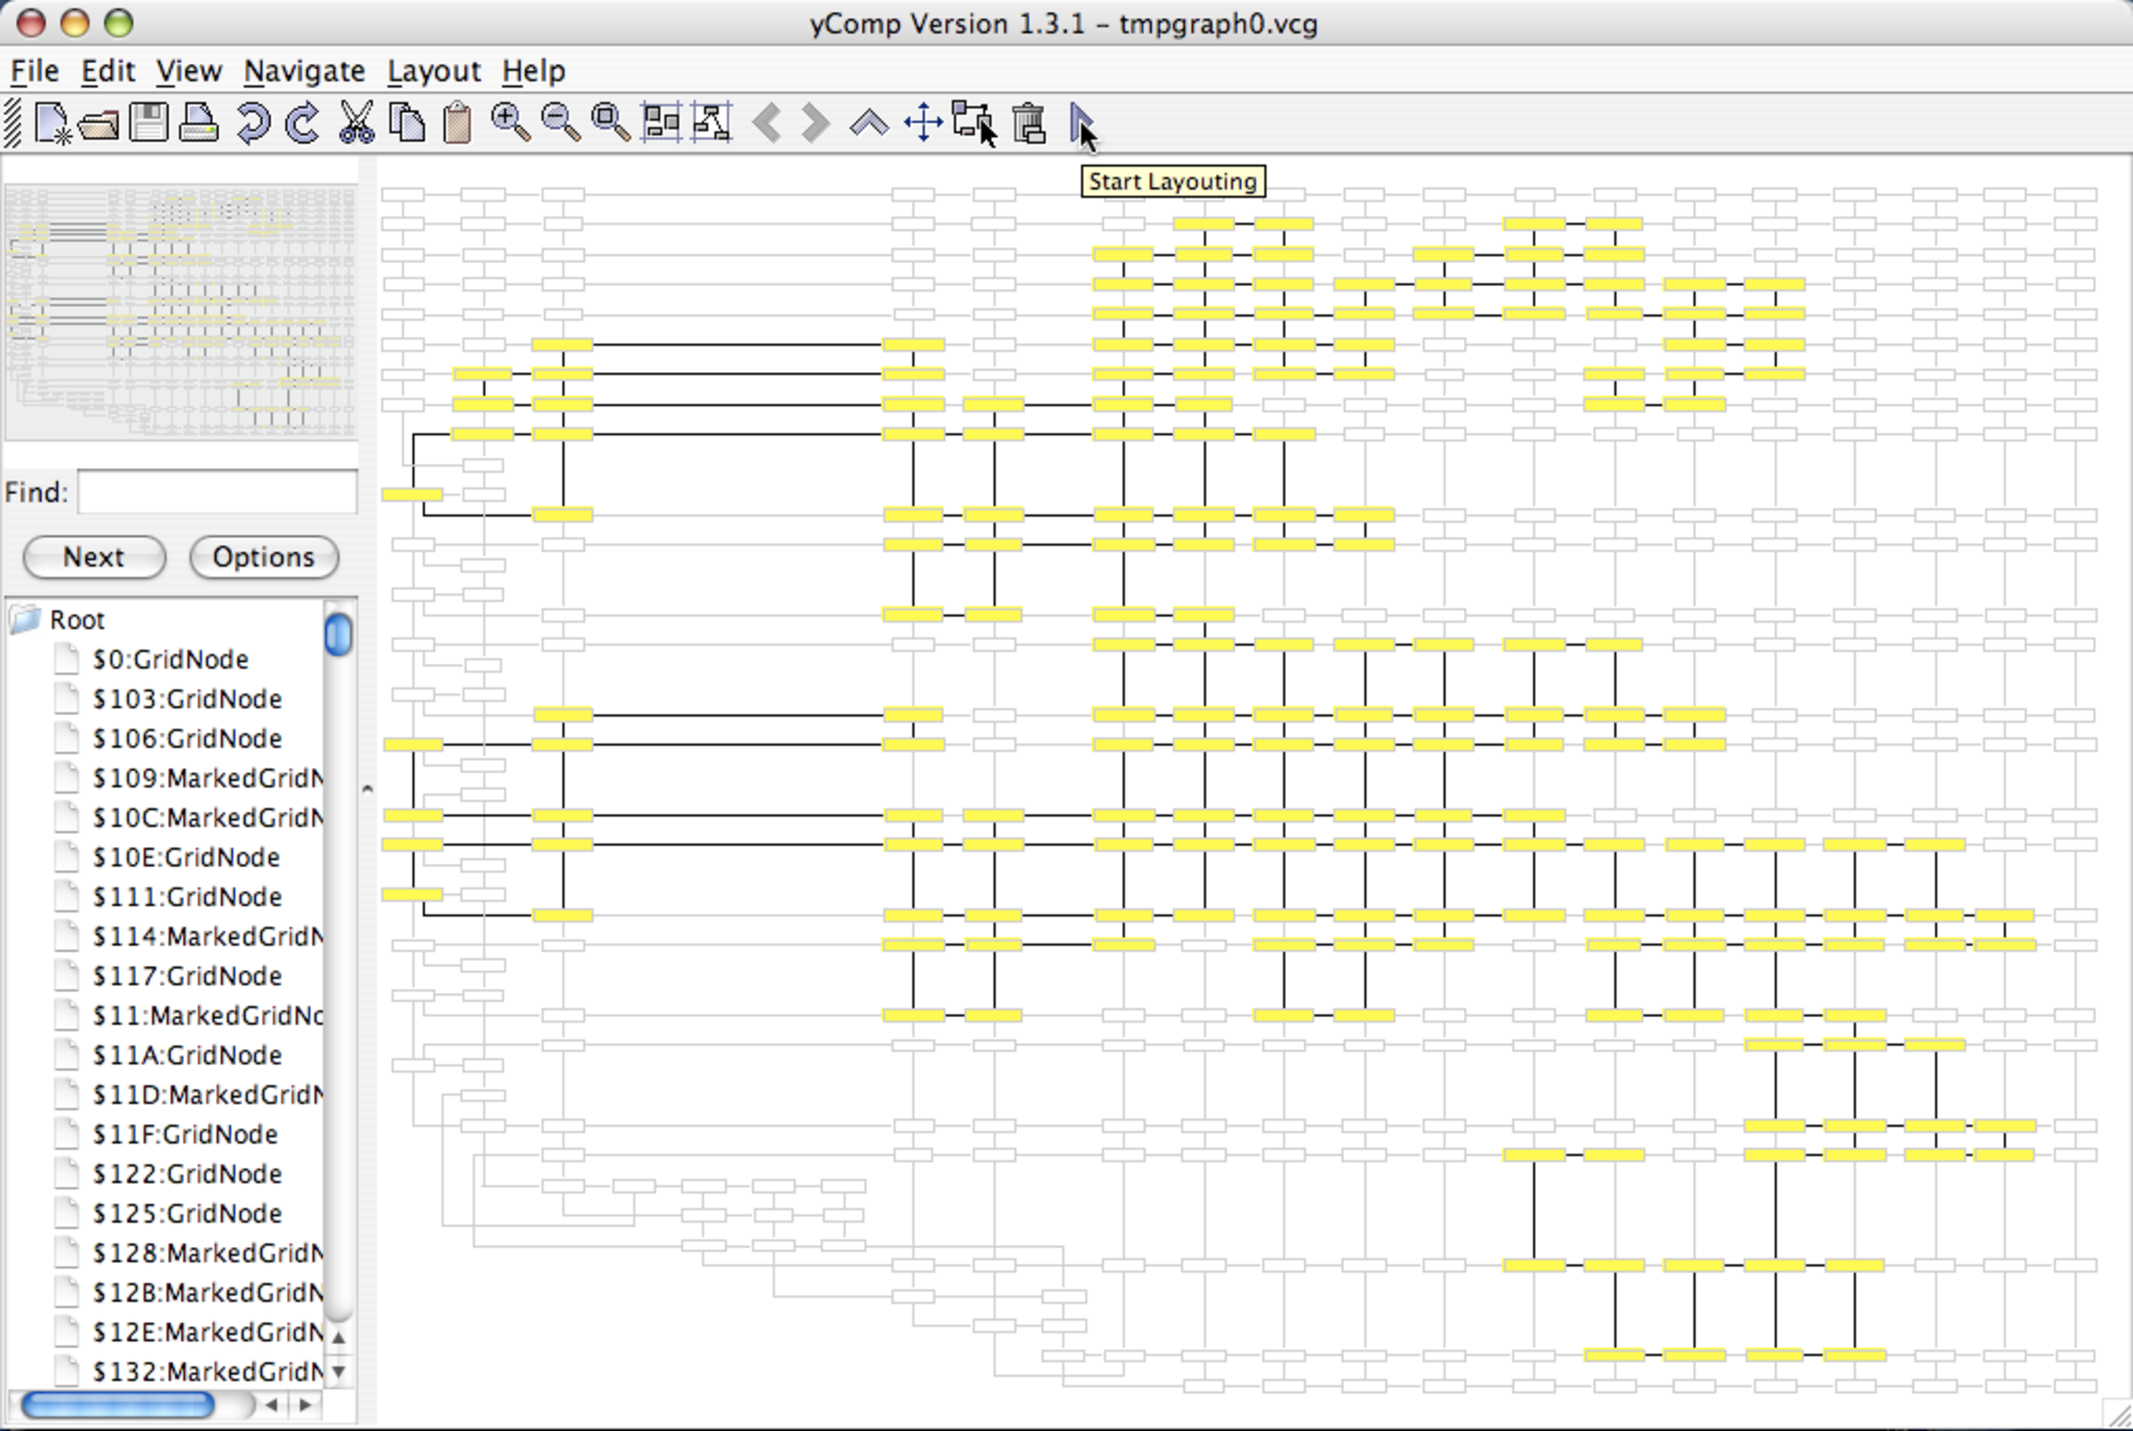
\includegraphics[width=0.45\linewidth]{fig/ycomp2.pdf}
\end{center}
  \item[Requires] Java Runtime Environment 1.5 (or above).
\end{description}


\section{Development goals}

The development goals of \GrG\ were

\begin{description}

\item[Expressiveness]
is achieved by powerful and declarative specification languages for pattern matching and rewriting by rewrite rules, builing upon a rich graph model language.
In addition to the unmatched expressiveness of the basic actions,
the rule language now offers nested and subpatterns which allow to handle substructures of arbitrary depth and arbitrary breadth declaratively within the rules,
by now even surpassing the capabilities of the VIATRA2\cite{viatra2,recursiveviatra} graph rewriting tool, the strongest competitor in rule expressiveness. 
The rules can be combined by graph rewrite sequences, a rule application control language with variables and logical as well as iterative control flow;
it was recently extended by storages as pioneered by the VMTS\cite{vmts} graph rewriting tool, allowing for more concise and faster solutions.

\item[Performance]
i.e. high speed at modest memory consumption, is needed to tackle real world problems.
It is achieved by typing, easening the life of the programmer by eliminating large classes or errors as well as speeding up the pattern matcher,
by the generative approach compiling the rules into executable code, 
and by the heuristic optimizations of search state space stepping and the host graph sensitive search plans.
In order to accelerate the matching step, we internally introduce \newterm{search plans} 
to represent different \newterm{matching strategies} and equip these search plans with a cost model, taking the present host graph into account.
The task of selecting a good search plan is then considered as an optimization problem~\cite{BKG:07,Bat:06}.
In contrast to systems like Fujaba\cite{fujaba,fuj}, our strongest competitor regarding performance, 
our pattern matching algorithm is fully automatic and does not need to be tuned nor to be implemented in parts by hand.
According to \indexed{Varr\'o's benchmark}\cite{varro_bench}, it is at least one order of magnitude faster than any other tool known to us.

\item[Development Convenience]
is gained by interactive and graphical debugging of the rule application, capable of visualizing the matched pattern, the rewrite which will be applied, and the currently active rule out of the rewrite sequence.
A further point easening development is the application programming interface of the generated code,
which offers access to named, statically typed entities, catching most errors before runtime and allowing the code completion mechanisms of modern IDEs to excel.
In addition a generic interface operating on name strings and .NET objects is available for applications where the rules may change at runtime (as e.g. the \GrShell).
Another important factor regarding development convenience is currently read by you.
There's one convenience not offered you may expect: a visual rule language and an editor.
This brings a clear benefit -- graph transformation specifications to be processed by \GrG\ can be easily generated --
but especially is a good deal cheaper to implement. Given the limited resources of an university project this is an important point,
as can be seen with the AGG\cite{agg} tool, offering a nice graphical editor but delivering performance only up to simple toy examples 
(causing the wrong impression in the heads of users that graph rewriting is notoriously inefficient).

\item[Well Founded Semantics]
to ease formal, but especially human reasoning.
The semantics of \GrG\ are specified in \cite{DissRuby}, based upon graph homomorphisms, denotational evaluation functions and category theory.
The \GrG-rewrite step is based by default on the \newterm{single-pushout approach} (SPO, for explanation see~\cite{spoapproach}),
with the \newterm{double-pushout approach} (DPO, for explanation see~\cite{dpoapproach}) available on request, too.
The semantics of the recursive rules introduced in version 2.0 are given in \cite{Jak:08},
utilizing pair star graph grammars on the meta level to assemble the rules of the object level.
The formal semantics are not as complete as for the graph programming language GP\cite{gp} though, mainly due to the large amount of features 
-- the convenience at using the language had priority over the convenience at reasoning formally about the language.

\item[Platform Independence]
is achived by using languages compiled to byte code for virtual machines backed by large, standardized libraries, specifically: Java and C\#.
This should prevent the fate of the grandfather of all graph rewrite systems, PROGRES\cite{schuerr99progres},
which achieved a high level of sophistication, but is difficult to run by now, or simply: outdated.

\item[General Purpose Graph Transformation]
in contrast to special purpose graph transformation.
A lot of other graph based tools are geared towards special purpose applications, 
e.g. verification (GROOVE \cite{Groove}), or biology (XL \cite{xl}, or model transformation (VIATRA2\cite{viatra2}).
This means that design decisions were taken to ease uses in this application areas at the cost of rendering uses in other domains more difficult.
And that features were added in a way which just satisfies the needs of the domain at hand instead of striving for a more general solution 
(which would have caused higher costs at designing and implementing this features).
While the old \textsc{GrGen} was built as a special purpose compiler construction tool for internal use 
(optimizations on the graph based compiler intermediate representation FIRM -- see \url{www.libfirm.org}), 
the new \GrG\ was built from the beginning as a general purpose graph transformation tool for external use
-- to be used in areas as diverse as computer linguistics, software engineering, computational biology or sociology --
for reasoning with semantic nets, transformation of natural language to UML models,
model transformation, processing of program graphs, genome simulation, or pattern matching in social nets. 
Several of them are worked on, you may have a look at \cite{usecomputerlinguistics} or \cite{usemodeltransformation} or \cite{usegeneexpression}.

\end{description}
